%% ****** Start of file aiptemplate.tex ****** %
%%
%%   This file is part of the files in the distribution of AIP substyles for REVTeX4.
%%   Version 4.1 of 9 October 2009.
%%
%
% This is a template for producing documents for use with 
% the REVTEX 4.1 document class and the AIP substyles.
% 
% Copy this file to another name and then work on that file.
% That way, you always have this original template file to use.

%\documentclass[aip,graphicx]{revtex4-1}
%\documentclass[aip,reprint]{revtex4-1}

%\usepackage{graphicx}

%\draft % marks overfull lines with a black rule on the right
%\documentclass[pre,aps,floatfix,authordate1-4,twocolumn]{revtex4-1}
%\documentclass[pre,aps,floatfix,authordate1-4]{revtex4-1}

\documentclass[aip,jcp,twocolumn]{revtex4}
%\documentclass[aip,jcp]{revtex4}
%\documentclass{article}



%\documentclass[aps,prl,preprint,groupedaddress]{revtex4}

\usepackage{rotating} 
\usepackage{times}
\usepackage{graphicx}
\usepackage{setspace}
\usepackage{amsmath}
\usepackage{epstopdf}
\usepackage[obeyFinal]{easy-todo}
\usepackage{csquotes}
\usepackage{mhchem}
\usepackage{chemfig}

%\usepackage{markdown} 

\begin{document}

% Use the \preprint command to place your local institutional report number 
% on the title page in preprint mode.
% Multiple \preprint commands are allowed.
%\preprint{}

\title{Accurate binding of sodium and calcium to phospholipid bilayers by effective inclusion of electronic polarization} %Title of paper

% repeat the \author .. \affiliation  etc. as needed
% \email, \thanks, \homepage, \altaffiliation all apply to the current author.
% Explanatory text should go in the []'s, 
% actual e-mail address or url should go in the {}'s for \email and \homepage.
% Please use the appropriate macro for the type of information

% \affiliation command applies to all authors since the last \affiliation command. 
% The \affiliation command should follow the other information.

\author{Josef Melcr}
\author{Hector Martinez-Seara}
\affiliation{Institute of Organic Chemistry and Biochemistry,
Academy of Sciences of the Czech Republic, 
Prague 6, Czech Republic}
\author{Ji{\v r}{\' i} Kolafa}
\affiliation{Department of Physical Chemistry, Institute of Chemical Technology, Prague 6, Czech Republic}
\author{Pavel Jungwirth}
\affiliation{Institute of Organic Chemistry and Biochemistry,
Academy of Sciences of the Czech Republic, 
Prague 6, Czech Republic}
\affiliation{Department of Physics, Tampere University of Technology, P.O. Box 692, FI-33101
Tampere, Finland}

\author{O. H. Samuli Ollila}
\email[]{samuli.ollila@helsinki.fi}
%\homepage[]{Your web page}
\affiliation{Institute of Organic Chemistry and Biochemistry,
Academy of Sciences of the Czech Republic, 
Prague 6, Czech Republic}
\affiliation{Institute of Biotechnology, University of Helsinki}


% Collaboration name, if desired (requires use of superscriptaddress option in \documentclass). 
% \noaffiliation is required (may also be used with the \author command).
%\collaboration{}
%\noaffiliation

\date{\today}

\begin{abstract}
  % insert abstract here
Binding affinities and stoichiometries of Na$^+$ and Ca$^{2+}$ ions to phospholipid
bilayers are of paramount significance in the properties and functionality of cellular
membranes. Current estimates of binding affinities and
stoichiometries of cations are, however, inconsistent due to limitations in the available experimental and
computational methods. In this work, we improve the description of the binding details of Na$^+$ and Ca$^{2+}$ ions to the
1-Palmitoyl-2-oleoyl-phosphatidylcholine (POPC) bilayer by implicitly including electronic
polarization as a mean field correction, known as the electronic continuum correction (ECC).
This is applied by scaling the partial charges of a selected state-of-the-art POPC lipid model for molecular dynamics simulations.
Our improved ECC-POPC model reproduces not only the
experimentally measured structural parameters for the ion-free membrane, but also the
response of lipid head group to a strongly bound cationic amphiphile, as well as the binding affinities of 
Na$^+$ and Ca$^{2+}$ ions. With our new model we observe on the one side negligible binding of Na$^+$ ions to POPC
bilayer, while on the other side stronger interactions of Ca$^{2+}$ primarily with phosphate oxygens, which is
in agreement with the previous interpretations of the experimental spectroscopic data.
The present model results in Ca$^{2+}$ ions forming complexes with one to three POPC molecules with almost
equal probabilities, suggesting more complex binding stoichiometries than those from simple models
used to interpret the NMR data previously.
The results of this work pave the way to quantitative molecular simulations with realistic electrostatic interactions 
of complex biochemical systems at cellular membranes.
\end{abstract}

%\pacs{}% insert suggested PACS numbers in braces on next line

\maketitle %\maketitle must follow title, authors, abstract and \pacs

% Body of paper goes here. Use proper sectioning commands. 
% References should be done using the \cite, \ref, and \label commands

\section{Introduction}
Interactions of ions with cellular membranes play a key role in many important biological processes~\cite{seelig90,cevc90}. Ions, especially multivalent cations, modify general properties of the membrane which also modulate the embedded transmembrane proteins~\cite{cevc90,tocanne90, pabst07}. For example, Ca$^{2+}$  is crucial in propagation of neural signals. It promotes membrane fusion by bridging lipids in the vesicles carrying neurotransmitters and the neuron synapsis membrane~\cite{REF}. Ca$^{2+}$ also participates in the T-cell receptor activation. It induces the detachment of the positively charged cytosolic tails of the CD3 protein complex from the negatively charged intracellular membrane making it accessible for the Lck protein~\cite{Shi2013Ca2}. Another example involving sugar-lipid interactions mediated by ions concerns Ca$^{2+}$ modulating the presentation of the sugars present in the PI(4,5)P$_2$ lipid which ultimately modulates the phospholipase C delta 1 pleckstrin homology domain (PLC $\delta$1-H)~\cite{Bilkova2017Calcium}. Interestingly, this effect is not present for Mg$^{2+}$, which illustrates the selectivity of these processes with respect to particular ions. Despite our increasing understanding of the role of ions in cell membrane-related processes the molecular details of the mechanisms behind such processes remain elusive in many cases. 

Direct measurements of ion-membrane interactions in complex biological systems are difficult. 
Hence, simplified lipid bilayers are often used as entry-level models to shed light on the role of ions in complex biological membranes~\cite{scherer87,seelig90,cevc90}. 
For this reason, interactions of biologically relevant cations, in particular Na$^+$ and Ca$^{2+}$, with zwitterionic phosphocholine (PC) bilayers have been widely studied experimentally~\cite{akutsu81, altenbach84, seelig90, cevc90, tocanne90, binder02, pabst07, uhrikova08} and using molecular dynamics (MD) simulations~\cite{bockmann03, bockmann04, Berkowitz12, melcrova16, javanainen17}. The details of ion binding are, however, not fully consistent in the literature. Non-invasive spectroscopic methods, like nuclear magnetic resonance (NMR), scattering, and infrared spectroscopies mostly suggest that Na$^+$ ions exhibit negligible binding to PC lipid bilayers. In contrast, Ca$^{2+}$ is observed to specifically bind to a couple of PC molecules via their phosphate groups~\cite{hauser76, hauser78, herbette84, akutsu81, altenbach84, binder02, pabst07, uhrikova08}. Most atomistic resolution MD simulation models predict stronger membrane bindings of the cations than observed in experiments~\cite{catte16}. Namely, simulations report various degrees of Na$^+$ accumulation at the lipid interface~\cite{bockmann03} and for Ca$^{2+}$ strong binding to up to four PC lipids simultaneously, involving not only interactions with phosphates but also with carbonyl oxygens~\cite{bockmann04, melcrova16, javanainen17}.

Recent studies within the NMRlipids project (\url{nmrlipids.blogspot.fi})~\cite{catte16} made an attempt to resolve these disagreements. A direct comparison of ion binding affinities to PC bilayers between simulations and experiments has been made possible using the electrometer concept~\cite{seelig87}. Namely, the changes in NMR order parameters of the head group upon addition of ions are directly compared to the MD simulations results. 
Analyzing massive amounts of data collected within an open collaboration approach, 
it was concluded that the accuracy of the current state-of-the-art lipid models for MD simulations is not sufficient for a detailed interpretation of the interactions of cations with PC lipid bilayers~\cite{catte16}.

In this work, we improve the description of cation binding to a POPC bilayer within MD simulations 
via an implicit inclusion of electronic polarizability in the polar region of phospholipids. 
To this end, we apply the electronic continuum correction (ECC)~\cite{leontyev11}, 
within which scaling of the atomic partial charges is employed to account for the missing electronic polarizability in standard force field MD simulations. 
Such an approach has been shown previously to improve the behavior of ions in simulations of aqueous salt solutions~\cite{martinek17, Pluharova2014, kohagen14, kohagen16}. Here, we extend the ECC approach to aqueous lipid membranes taking the Lipid14 force field~\cite{dickson14} as a starting point for refining the POPC model. This choice is justified by the fact that the Lipid14 provides the least inaccurate descriptions of cation binding among the existing force fields\cite{catte16}. 
The newly developed ECC-POPC model reproduces the experimentally
measurable structural parameters of an ion-free POPC lipid bilayer with the accuracy comparable to the best state-of-the-art lipid models, while at the same time significantly improving the membrane binding affinities of sodium and calcium cations.

\section{Methods}

\subsection{Electronic continuum correction for lipid bilayers}\label{section:ecc}
The lack of electronic polarizability in standard MD force fields has been considered a serious issue since the early days of lipid bilayer simulations. In this work, we circumvent the demanding explicit inclusion of electronic polarization effects~\cite{lucas12, chowdhary13} by accounting for the electronic part of polarizability in lipid bilayer simulations implicitly via the electronic continuum correction (ECC)~\cite{leontyev11}. Technically, this is similar to the phenomenological charge-scaling applied in earlier studies of surfactants, lipids or ionic liquids \cite{jonsson86, egberts94, beichel14}. However, the present concept of ECC is physically well justified and rigorously derived~\cite{leontyev09, leontyev10, leontyev11, leontyev14}.

According to ECC, the electronic polarizability can be included into non-polarizable MD in a mean-field way by 
embedding the ions in a homogeneous dielectric continuum with a dielectric constant $\epsilon_{el}$, which is the electronic part of the dielectric constant of the medium~\cite{leontyev11}. Following Coulomb's law,  ECC can be directly incorporated by scaling the charges with a constant scaling factor of $f_q = \epsilon _{el} ^{-1/2}$, yielding
\begin{equation}
Q^{ECC} = f_q \cdot Q
\end{equation}
for the ECC corrected charges. 
Given that the  high frequency dielectric constant of water is $\epsilon _{el} = 1.78$ (\textit{i.e.,} the square of the refraction index), the scaling factor for ions in water is roughly $f_q \approx 0.75$. This scaling factor significantly improves the accuracy of simulations of solvated ions, when quantitatively compared with neutron scattering data \cite{kohagen14,kohagen16, Pluharova2014, martinek17}.
It is important to note that the value of the
high frequency dielectric constant 
is around 2 for almost any biologically relevant environment \cite{leontyev11}.
The dielectric discontinuity in a lipid bilayer thus arises only
from the nuclear (orientational) polarization of the molecules, which is accounted for explicitly in standard MD simulations. 
Therefore, the same correction for the electronic polarizability can be 
applied throughout the lipid bilayer/aqueous solution interface.

While using the scaling factor of $f_q = 0.75$ for ions in water is well justified in the ECC theory \cite{leontyev11}, it is not clear whether the same factor should be applied to partial charges used to describe molecules in MD models, e.g., lipids in our case. Unlike the total charge of an ion, atomic partial charges within molecules are not physical observables. Several schemes exist for the assignment of partial charges for biomolecules~\cite{Hu2007}, with the restrained electrostatic potential method (RESP) being commonly used~\cite{RESP_paper, Singh1984}. Considering that water is often included in RESP calculations or charges are refined to improve certain experimental observables, the electronic polarizability effects of the solvent may to some extent be included in standard force fields~\cite{RESP_paper, Singh1984, jorgensen96, ipolq2013, benavides17}. Thus, our application of the scaling factor, $f_q$, to existing partial charges in molecules does not necessarily follow $f_q = \epsilon _{el} ^{-1/2}$. Instead, a consistent scaling factor should lie between the value of 0.75  (\textit{i.e.,} no electronic polarizability included in the original partial charges) and 1 (\textit{i.e.,} electronic polarizability fully included in the original partial charges). 

Here we develop a ECC-POPC lipid model that accurately describes binding 
of sodium and calcium ions to the POPC  lipid bilayer. 
The Lipid14~\cite{dickson14} force field 
(available in a Gromacs format from Ref. \citenum{lipid14files}) was used as a starting 
point since 
it provides the most accurate response of the head groups to ions among the available 
lipid models (see Figs.~2~and~5 in Ref.~\citenum{catte16}). Additionally, the Lipid14 model 
provides realistic head group, glycerol backbone, and acyl chain structures~\cite{dickson14,botan15}.
We applied the ECC correction 
to the Lipid14 model of POPC by scaling 
partial charges of the head group, glycerol 
backbone, and carbonyl regions. 
These are the polar parts of phospholipids which can 
contribute to the cation binding. 

To reproduce the experimental ion binding affinities,
we scanned possible values of the scaling factor from the interval $f_q~\in~(0.75, 1.0)$.
The ion binding affinity was benchmarked against experiments
using the head group order parameters and the electrometer concept \cite{seelig87,catte16},
as discussed more detail in the next section.
Scaling down the partial charges reduced the ion binding affinity.
We found the most accurate ion binding affinities with a scaling factor of $f_q = 0.8$,
which is only slightly higher than the ECC one ($f_q=0.75$).
Directly applying
the 0.8 scaling to the partial charges of the head group, the glycerol backbone, and
the carbonyls reduced the area per lipid to 60~\AA$^2$. This area is smaller than in the
original Lipid14 model ($65.6 \pm 0.5$~\AA$^2$)~\cite{dickson14} and in experiments
(64.3~\AA$^2$) \cite{kucerka11}. The decrease of the area per lipid arises from a
reduced hydration of the lipid head group region after scaling of the partial charges, which effectively
reduces the head group polarity. We solve this problem by slightly reducing the effective radii of
the modified head group atoms via lowering the $\sigma$ parameters in the Lennard-Jones potential by a
factor of $f_\sigma = 0.89$. The same approach was successfully adopted for the ECC ions in aqueous
solutions previously \cite{kohagen14, kohagen16, Pluharova2014, martinek17}. After reducing the head group atoms $\sigma$ parameters, the area per molecule is restored to the experimental value (Table~\ref{tab:apls}). 




\subsection{Electrometer concept} \label{section:electrometer}
Comparing MD simulation to NMR experiments, we can validate the ion
binding affinity in lipid bilayer simulations using the 'electrometer concept'~ \cite{seelig87, catte16}.
This method is based on the experimental observation that the C-H bond order parameters of $\alpha$ and $\beta$ carbons in a PC lipid head group (Fig.~\ref{simVSexpNOions}) are proportional to the amount of charge bound per lipid~\cite{seelig87}.
The order parameters for all C-H bonds in lipid molecules can be accurately measured using $^2$H NMR or $^{13}$C NMR techniques \cite{ollila16}. From MD simulations the order parameters can be calculated using the relation
\begin{equation}\label{OP}
S_{\rm CH}=\frac{3}{2}\langle \cos^2\theta -1 \rangle,
\end{equation}
where $\theta$ is the angle between the C-H bond and the membrane normal. Angular brackets point to the average over all sampled configurations.

The relation between the amount of the bound charge per lipid, $X^\pm$, and the head group order parameter change, $\Delta S_{\rm{CH}}^{i}$, is empirically quantified as~\cite{seelig87,ferreira16}
\begin{equation}\label{OPchangeEQ}
\Delta S_{\rm{CH}}^{i}= S_{\rm{CH}}^{i}(X^\pm)-S_{\rm{CH}}^{i}(0) \approx m_i \frac{4 }{3\chi}X^\pm,
\end{equation}
where $i$ refers to either the $\alpha$ or $\beta$ carbons, $S_{\rm{CH}}^{i}(0)$ denotes the order parameter in the absence of bound charge, $\chi$ is the quadrupole coupling constant ($\chi \approx$\,167\,kHz), and $m_i$ is an empirical constant depending on the valency and location of the bound charge.


The measured change of the order parameter depends on the head group response to the bound charge and on the amount of the bound charge (\textit{i.e.,} $m_i$ and $X^\pm$ in Eq.~\ref{OPchangeEQ}, respectively).  The empirical factor $m_i$ has to be adequately quantified before the electrometer concept can be used to analyze the binding affinities. This calibration has been done experimentally for a wide range of systems~\cite{seelig87, beschiasvili91}. To calibrate the response of the head group order parameters to the bound charge in simulations, we use experimental data for a strong cationic surfactant dihexadecyldimethylammonium bromide  (DHAB) mixed with a POPC bilayer~\cite{scherer89}. DHAB\\[0.5cm]
%\vspace{0.5cm}
\chemfig{
  -[:0,3.5,,,draw=none]\chemabove{N}{\scriptstyle\oplus} (-[:150]H_3C)(-[:210]H_3C)(-[:330]{(}CH_2{)}_{15}-CH_3)(-[:30]{(}CH_2{)}_{15}-CH_3)
}  
\vspace{0.5cm} \\
is a cationic surfactant having two acyl chains and bearing a unit charge at the hydrophilic end. Due to its structure it is expected to locate in the bilayer similarly to the phospholipids and its molar ratio then gives directly the amount of bound unit charge per lipid $X^\pm$ in these systems~\cite{scherer89}.

\subsection{Salt concentrations and binding affinities}
When measuring head group order parameters, the NMR experiments report the employed salt concentrations in two different ways.
Some studies provide the salt concentrations in water before solvating the lipids~\cite{akutsu81}, $C_{ion}'$,
while others use atomic absorption spectroscopy and report the salt concentration in
the supernatant after the solvation of lipids~\cite{altenbach84}, $C_{ion}$. In this work,
we stick to the latter definition by estimating the salt concentration in the aqueous
bulk region using the farthest point from the lipid bilayer in the aqueous phase.
Note that the former definition was used by some of us previously.~\cite{catte16}.
Although these two definitions provide somewhat different values when applied
to Ca$^{2+}$ concentrations, their particular choice does not affect the conclusions of this work in any significant way.

To quantify the ion binding affinities to a lipid bilayer, we calculate the relative surface excess of ions with respect to water, $\Gamma_{ion}^{water}$~\cite{chattorajBOOK}. Such a quantity compares the adsorption of ions to the adsorption of water molecules at the interface without the necessity of defining a Gibbs dividing surface between the membrane interior and the water bulk region. In our simulations, we only assume that the interface is located between the ion-free hydrophobic interior of the lipid bilayer and the aqueous region far from the membrane.  Such a setup and the above definition of bulk ion concentrations provides a simple relation for the relative surface excess $\Gamma_{ion}^{water}$ for simulations of lipid bilayers,
 \begin{equation}\label{surfexcess}
  \Gamma_{ion}^{water}=\frac{1}{2A_b} \left ( n_{ion} - n_{water} \frac{C_{ion}}{C_{water}} \right ).
\end{equation}
Here, $n_{water}$ and $n_{ion}$ are the total numbers of water molecules and ions in the system,
$C_{water}$ and $C_{ion}$ are their respective bulk concentrations in the aqueous phase,
and $A_b$ is the area of the unit cell in the membrane plane.
The total area of the interface is then twice the area of the membrane, i.e., $2A_b$,
because the bilayer has an interface at each of the two leaflets.



\subsection{Validation of lipid bilayer structure against NMR and scattering experiments}
The structures of lipid bilayers in simulations without ions were validated against NMR by calculating the order parameters for the C-H bonds and against \mbox{X-ray} scattering experiments by evaluating the scattering form factors. NMR order parameters validate the structures sampled by the individual lipid molecules with atomic resolution. The simulated order parameters were calculated for all C-H bonds in lipid molecules from Eq. \ref{OP}. Scattering form factors validate the dimensions of the lipid bilayer (i.e., the bilayer thickness and area per molecule). Form factors were calculated using a relation

\begin{equation}
  F(q) = \int _{-D/2} ^{D/2} \left ( \rho_{el}(z) - \rho_{el}^s \right ) \cos (zq_z) \mathrm{d}z,
  %F(q) = \int _{-D/2} ^{D/2} \left ( \sum _\alpha f_\alpha (q_z) n_\alpha (z) - \rho _s \right ) \exp (izq_z) \mathrm{d}z,
\end{equation}

\noindent where $\rho_{el} (z)$ is the total electron density, $\rho_{el}^s$ is the electron density of the solvent far in the aqueous bulk, and $z$ is the distance from the membrane center along its normal with $D/2$ being half of the unit cell size.  




\subsection{Simulation details}

\subsubsection{Simulations of POPC bilayers with aqueous ions}
Simulations of a POPC bilayer in pure water or at varying salt concentrations consisted of 128 POPC molecules
and approximately 50~water molecules per lipid in an orthorhombic simulation box with periodic boundary conditions.
The SPC/E~\cite{Berendsen1987} water model was used in all ECC-POPC model simulations reported
in the main text. This model was also used in the previous parametrization
of ECC-ions \cite{martinek17, kohagen16, Pluharova2014} because its lowered dielectric constant is consistent with
the ECC concept~\cite{leontyev11, leontyev14}.
The robustness of our approach with other water models (OPC \cite{Izadi14},
OPC3~\cite{Izadi16}, TIP3P~\cite{jorgensen83}, TIP3P-FB and TIP4P-FB~\cite{Wang2014}, and TIP4P/2005 \cite{Abascal2005})
was verified and is presented in the Supporting Information (SI).
Sodium, calcium, and chloride ions were modeled as ECC-ions
with parameters from Refs. \citenum{martinek17, Pluharova2014}. Scaled charges and Lennard-Jones radii for atoms
forming the POPC lipid were derived in this work starting from the Lipid14 force field~\cite{dickson14}.
For comparison, simulations with the Lipid14 model~\cite{dickson14} and
ion models by Dang and coworkers~\cite{smith94,chang1999,dang2006} or ECC-ions \cite{martinek17, kohagen16, Pluharova2014}
were also performed. The TIP3P water model~\cite{jorgensen83} was used in all simulations with the original Lipid14 model.
Simulation data for the Lipid14 model with \AA{}qvist ions~\cite{aqvist90} and the TIP3P~\cite{jorgensen83} water model were taken directly from
Refs.~\citenum{catte16,lipid14POPC0mMNaClfiles,lipid14POPC350mMCaClfiles,lipid14POPC350mMCaClfilesNC,lipid14POPC1000mMNaClfiles}.  

MD simulations were performed using the GROMACS \cite{Abraham15} simulation package (version 5.1.4). The simulation parameters used
in this work are summarized in Table~S1 in the SI. 
Compatibility with the openMM simulation package \cite{openmm7} was also
tested and is presented in the SI. 
The simulated trajectories and parameters files are available at \cite{??} \todo{To be uploaded to Zenodo}.



\subsubsection{Simulations of POPC bilayers with cationic surfactants}
The topology of the dihexadecyldimethylammonium cation was created with the automated topology builder \cite{malde11}. The AmberTools program~\cite{amber} was used to generate the Amber-type force field parameters. These parameters were then converted to the Gromacs format with the acpype tool \cite{acpype}. The partial charges were manually modified in the non-scaled version to approximately match similar segments in Lipid14 \cite{dickson14}. For simulation with ECC-POPC, the partial charges of the head group of the cation were scaled by a factor of $f_q=0.8$, and the $\sigma$ of the scale atoms reduced by a factor of 0.89 similarly as for POPC-ECC.

The cationic surfactants were randomly mixed among the phospholipids to form bilayer structures with mole fractions of 10\%, 20\%, 30\%, 42\%, or 50\% of surfactant in the POPC bilayer. All these systems contained 50 POPC molecules per leaflet, 6340 water molecules, and 6, 14, 21, 35, or 50 surfactants per leaflet.  Chloride counter ions were used in all the simulations, while bromide was the counter ion in the experiment~\cite{scherer89}. For POPC, either Lipid14 with TIP3P~\cite{jorgensen83} or ECC-POPC with SPC/E~\cite{Berendsen1987} parameters  were used. The first 20~ns of the total simulation time of 200~ns was considered as an equilibration period and was thus omitted from the analysis. We checked that a sufficient lipid  exchange occurred during the simulations.
The trajectories and simulation files for unscaled systems are available from
Refs.~\citenum{POPClipid14T313K,POPClipid1410perCATsurfT313K,POPClipid1420perCATsurfT313K,POPClipid1430perCATsurfT313K,POPClipid1442perCATsurfT313K,POPClipid1450perCATsurfT313K}.

\todo{Provide the parameters for ECC-surfactant somewhere.
      Joe: They will appear along with the Zenodo upload of the trajectories.}

\section{Results and Discussion}

\subsection{Structural parameters of a pure ECC-POPC model membrane: Agreement with experiments}

\begin{figure}[tb!]
  \centering
  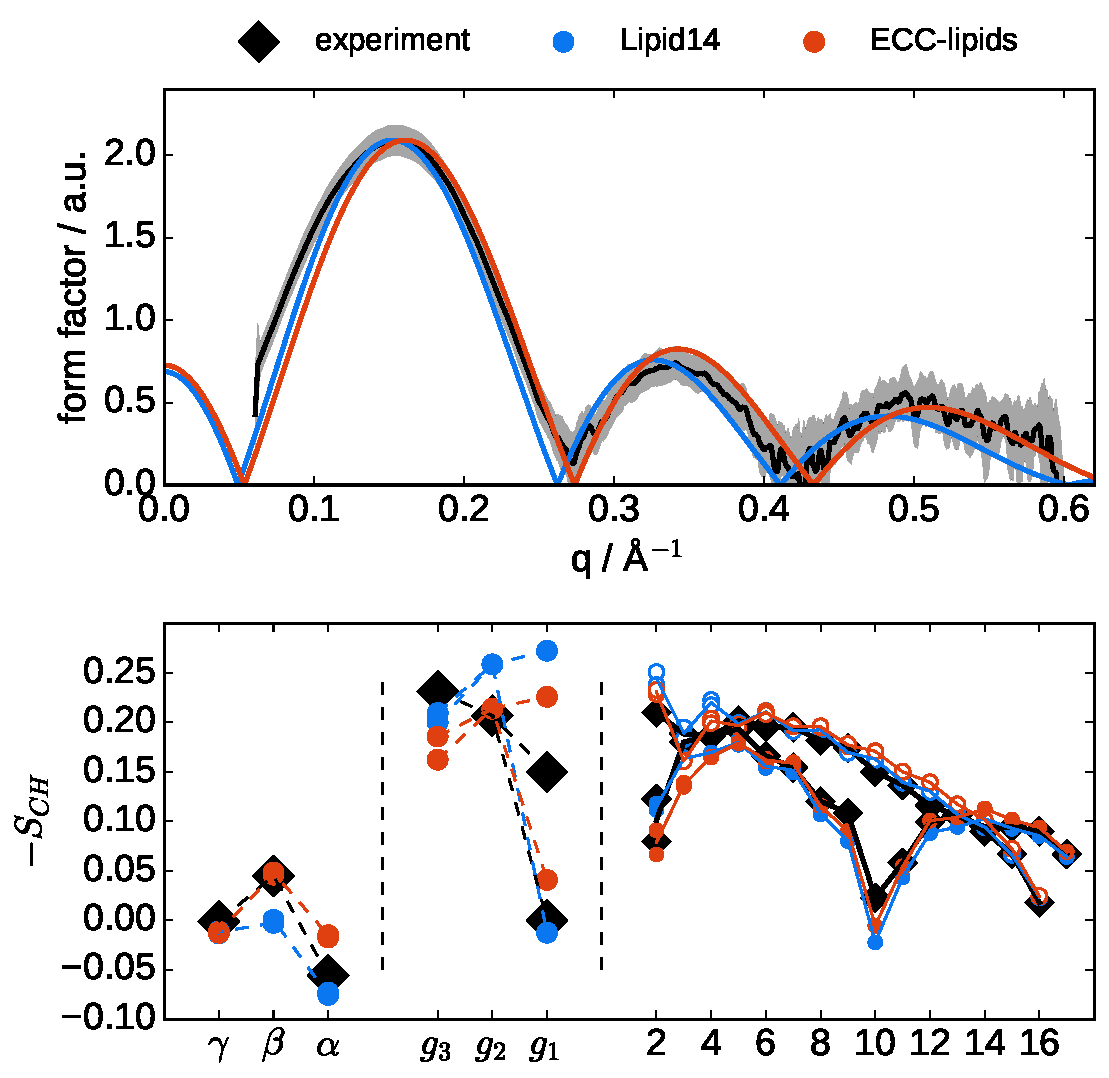
\includegraphics[width=8.2cm]{../Fig/ipython_nb/Order-parameters_form-factors_exp-L14-ECCL17_q80_sig89.pdf}
  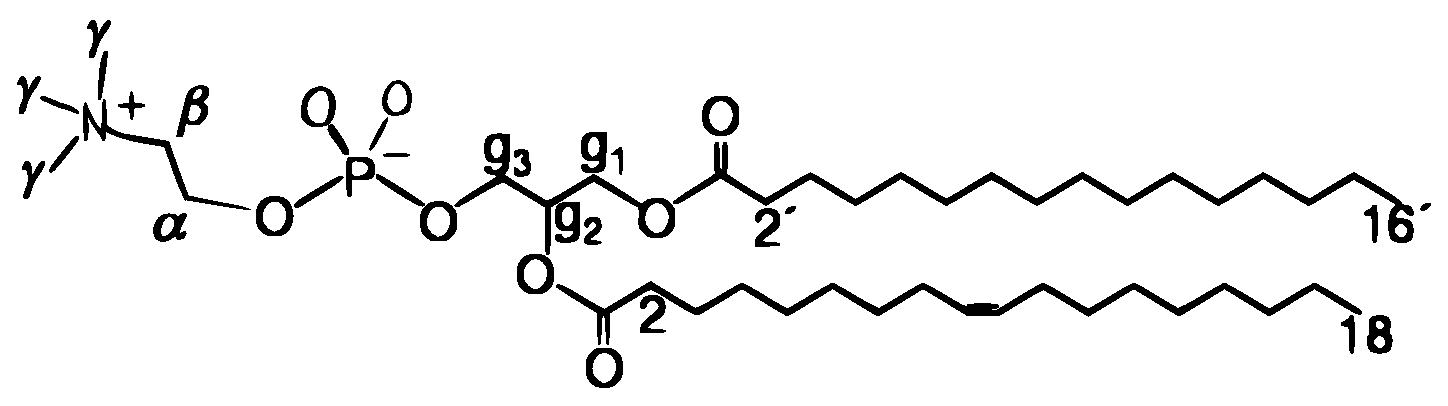
\includegraphics[width=7.4cm]{../Fig/POPCstructure.eps}
  %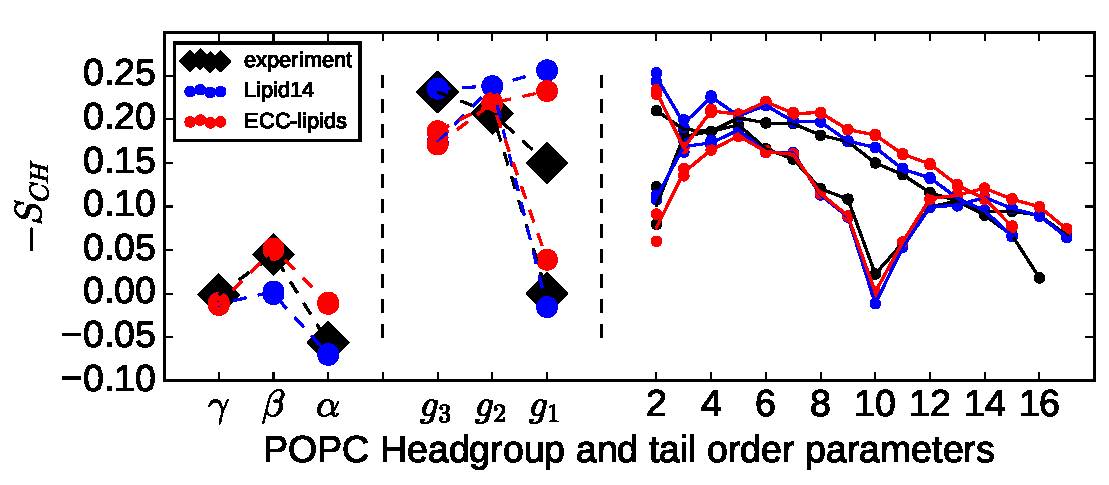
\includegraphics[width=8.0cm]{../Fig/ipython_nb/Order-parameters_exp-L14-ECCL17_q80_sig89.pdf}
  %\includegraphics[height=8.4cm,angle=-90]{../Fig/form-f_exp-l14-eccl17.eps}
  \caption{\label{simVSexpNOions}
    Top: X-ray scattering form factors from simulations with the Lipid14 \cite{dickson14} and
    the ECC-POPC models compared with experiments~\cite{kucerka11} at 303~K.
    Middle: Order parameters of POPC head group, glycerol backbone and acyl chains 
    from simulations with the Lipid14 \cite{dickson14} and the ECC-POPC models
    compared with experiments \cite{ferreira13} at 300~K.
    The size of the markers for the head group order parameters correspond to
    the error estimate $\pm 0.02$ for experiments \cite{botan15,ollila16},
    while the error estimate for simulations is $\pm 0.005$.
    The size of the points for acyl chains are decreased by a factor of 3 to improve the clarity of the plot.
    Bottom: The chemical structure of POPC and the labeling of the carbon segments.
  } 
    \todo{Joe: I'm fine with the name change from ECC-lipids to ECC-POPC, but we have to be consistent throughout the text. I changed all accurences of ECC-lipids to ECC-POPC in the text, I yet need to change all figure legends then.}
\end{figure}

\begin{table}[tb!]
  \caption{Values of the area per lipid (APL) of POPC bilayers without ions. \label{tab:apls}
  }
  \begin{tabular}{l|c c}
    model          & APL (\AA$^2$)   & Temperature [K] \\
    \hline
    Lipid14                   & 65.1$\pm$ 0.6  &  300 \\
    Lipid14 \cite{dickson14}  & 65.6$\pm$ 0.5  &  303 \\
    \hline
    ECC-POPC                & 63.2$\pm$ 0.6  &  300       \\
    \hline
    experiment \cite{kucerka11} & 64.3  &  303    \\
    \hline
  \end{tabular}
\end{table}


First, we present results for bilayers in pure water.
The ECC-POPC and Lipid14 models both reproduce the experimental X-ray scattering form factors
of a POPC bilayer with a comparable accuracy (see Fig.~\ref{simVSexpNOions}).
The area per lipid from the Lipid14 model is $\approx$1\AA{} larger than the
experimental value in Table~\ref{tab:apls}, while the value from the ECC-POPC model
is $\approx$1\AA{} smaller than the experimental one.
The values of the area per lipid of the ECC-POPC model vary slightly
when simulated with different water models (i.e., within the interval of 62.2--66.8 \AA{}, see Table~S2 in SI),
while still being close to the experimentally reported values.
We can thus conclude that the ECC-POPC model reproduces the experimental dimensions of the POPC
lipid bilayer with a comparable accuracy to other state-of-the-art lipid models~\cite{ollila16}.


Similarly, the acyl chain order parameters of the ECC-POPC model, as well as those of the Lipid14 model~\cite{dickson14}, agree with the experimental values within the error bars, as presented in Fig.~\ref{simVSexpNOions}. Notably, the experimentally measured forking and small order parameter values of the $C_2$ segment in {\it sn}-2 chain are well reproduced by both models. This feature has been suggested to indicate that the carbonyl of the {\it sn}-2 chain is directed towards the water phase, in contrast to the carbonyl in the {\it sn}-1 chain, which orients more along the bilayer plane~\cite{seelig75,schindler75,gawrisch92}.
This arrangement, which is not fully reproduced by other available lipid models~\cite{ollila16}, may be a relevant feature for the ion binding details.

The order parameters of the $\alpha$ and $\beta$ carbons in the head group are slightly larger in the ECC-POPC model than in the Lipid14 model, which is apparently related to the P-N vector orienting by about 7$^{\circ}$ more toward the water phase in the former model, see Fig.~\ref{OrderParameterCHANGESsurf}. While both models perform satisfactorily, considering the available experimental evidence, it is not possible to decide which of the two models provides more realistic head group orientations. The ECC-POPC model gives the $\beta$ carbon order parameter value closer to experiments than the Lipid14 model, while the opposite is true for the $\alpha$ carbon. The accuracy of both models in the glycerol backbone region is comparable to other state-of-the-art lipid model available in literature \cite{botan15}, see Fig.~\ref{simVSexpNOions}.


\todo{Dynamics check is missing: MSD (Hector/Joe)}

\subsection{Calibration of head group response to membrane-bound charge using cationic surfactant}\label{section:boundCHARGE}

\begin{figure}[tb!]
  \centering
  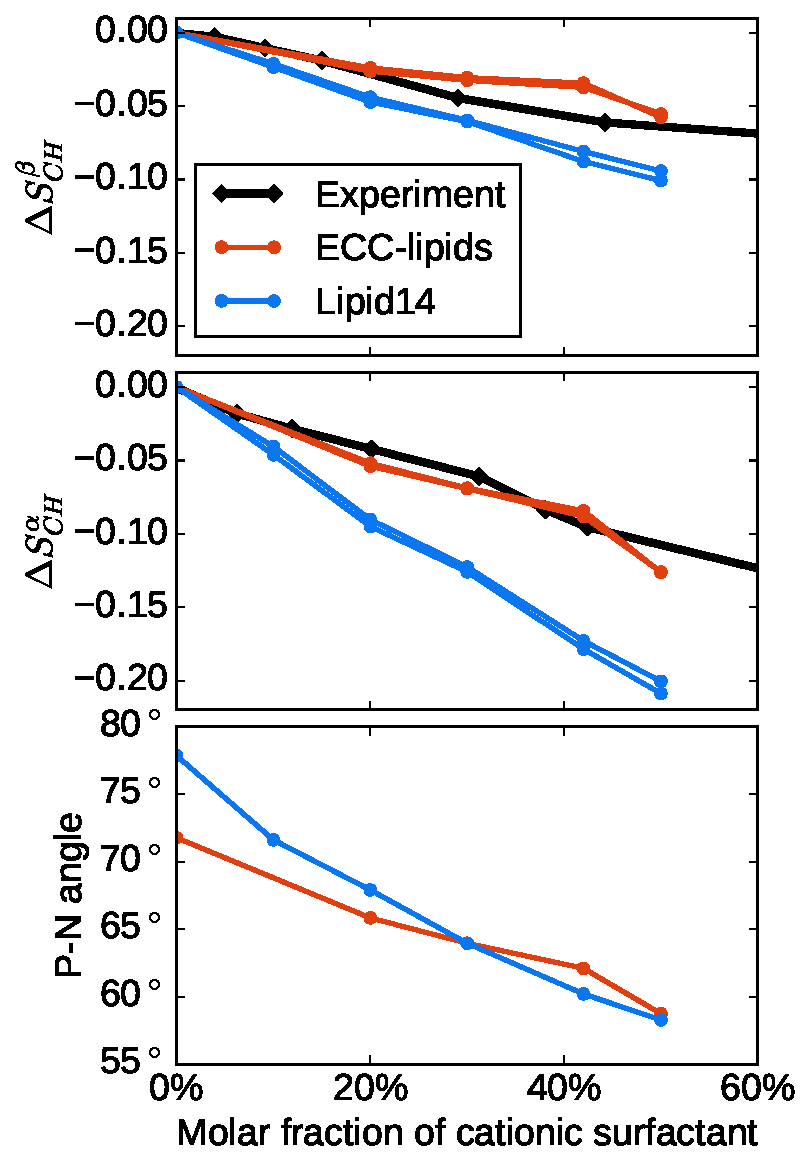
\includegraphics[width=8.0cm]{../Fig/ipython_nb/PN_angle_OrdPars-A-B_L14-ECCL17_q80_sig89_surf.pdf}
  \caption{\label{OrderParameterCHANGESsurf}
    The changes of head group order parameters and P-N vector orientation as a function of
    a molar fraction of the cationic surfactant dihexadecyldimethylammonium in a POPC bilayer
    from simulations and experiments \cite{scherer89} at 313 K.
  }
\end{figure}

Before studying the sodium and calcium ion binding affinities, we quantify the response of the head group order parameters to the amount of bound charge by using mixtures of monovalent cationic surfactants (dihexadecyldimethylammonium) and POPC~\cite{scherer89}. These mixtures have a well-defined amount of bound charge per PC, namely, the molar fraction of cationic surfactants. This is due to the ability of dihexadecyldimethylammonium to directly insert in the lipid bilayer due to its two hydrophobic acyl chains. Furthermore, available experimental data for these systems can be used to validate the sensitivity of lipid head group order parameters to the amount of bound charge in simulations \cite{scherer89}.

The changes of the head group order parameters with increasing amount of the cationic surfactant are compared between simulations and experiments~\cite{scherer89} in Fig.~\ref{OrderParameterCHANGESsurf}. An approximately linear decrease of the order parameters, as expected from Eq. \ref{OPchangeEQ}, is observed in both simulations and experiments at least for mole fractions below $\sim$30\%. The slope is, however, too steep in the Lipid14 model indicating that the response of head group order parameters to the bound positive charge is too strong. In contrast, the slope of the ECC-POPC model is in a very good agreement with experiments for the $\alpha$ segment, while being only slightly underestimated for the $\beta$ segment.

In Fig.~\ref{OrderParameterCHANGESsurf}, we show the headgroup P-N vector angle as a function of the mole fraction of the cationic surfactant. As suggested previously~\cite{seelig87}, the headgroup orients more towards the water phase with the increasing amount of positive charge in the PC lipid bilayer. The effect is more pronounced in the Lipid14 model than in the ECC-POPC model.   For example, the addition of 50\% mole fraction of the cationic surfactant leads to a decrease of 20$^{\circ}$ of the P-N vector angle for the Lipid14 model while only of 11$^{\circ}$ in the ECC-POPC model. The difference is in line with the smaller order parameter changes and the reduced charge--dipole interactions in the latter model. The weaker sensitivity of the P-N vector angle response in the ECC-POPC model is in better agreement with experiments.


\subsection{Validation of ECC-POPC model using binding affinities to Na$^+$ and Ca$^{2+}$ cations: the electrometer concept}


\begin{figure}[htb!]
  \centering
  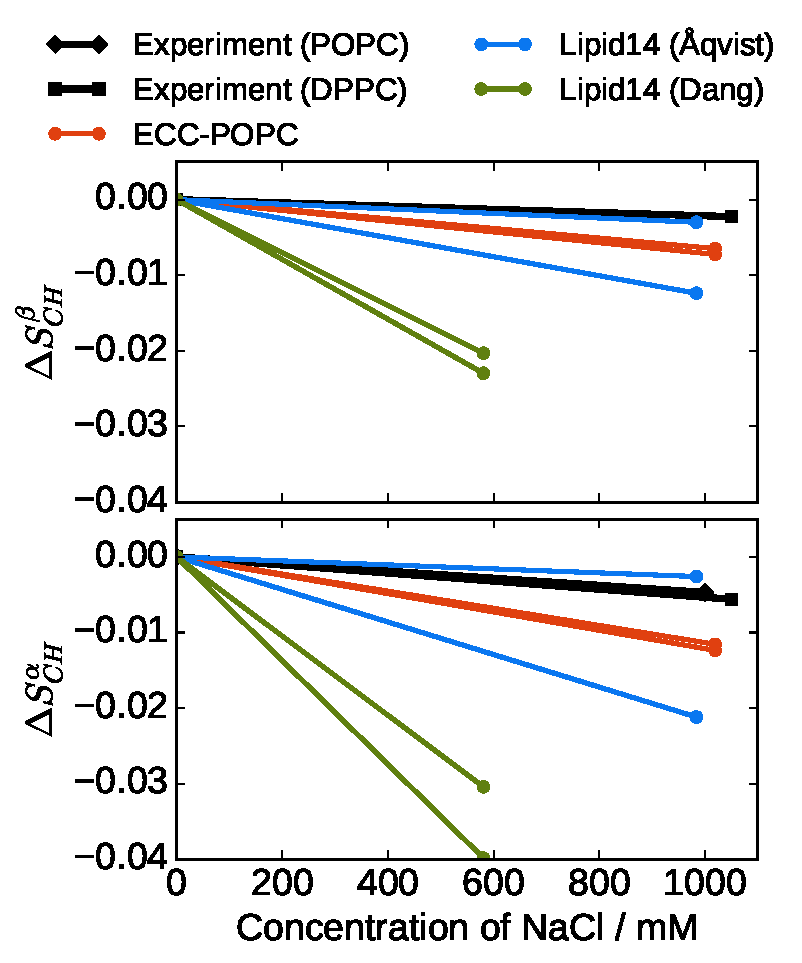
\includegraphics[width=8.0cm]{../Fig/ipython_nb/OrdPars-A-B_L14-ECCL17_q80_sig89_NaCl.pdf}
  \caption{\label{fig:delta_ordPar_NaCl}
    Changes of the head group order parameters of a POPC bilayer as a function of NaCl concentration
    in bulk ($C_{ion}$) from simulations with different force fields at 313 K together with 
    experimental data for DPPC (323\,K) \cite{akutsu81} and POPC (313\,K) \cite{altenbach84}.
    %Ion concentrations in x-axis are calculated as in Fig.~\ref{fig:delta_ordPar_CaCl}.
    Simulation data with Lipid14 and \AA{}qvist ion parameters at 298 K are taken directly from
    Refs.~\cite{lipid14POPC0mMNaClfiles,lipid14POPC1000mMNaClfiles}.
  }
  %Figure. in Ref.\cite{altenbach84} gives for POPC at 1M of NaCl $\Delta S^\alpha=(6.1-5.5)*0.00784=0.004704$.
\end{figure}

\begin{figure}[htb!]
  \centering
  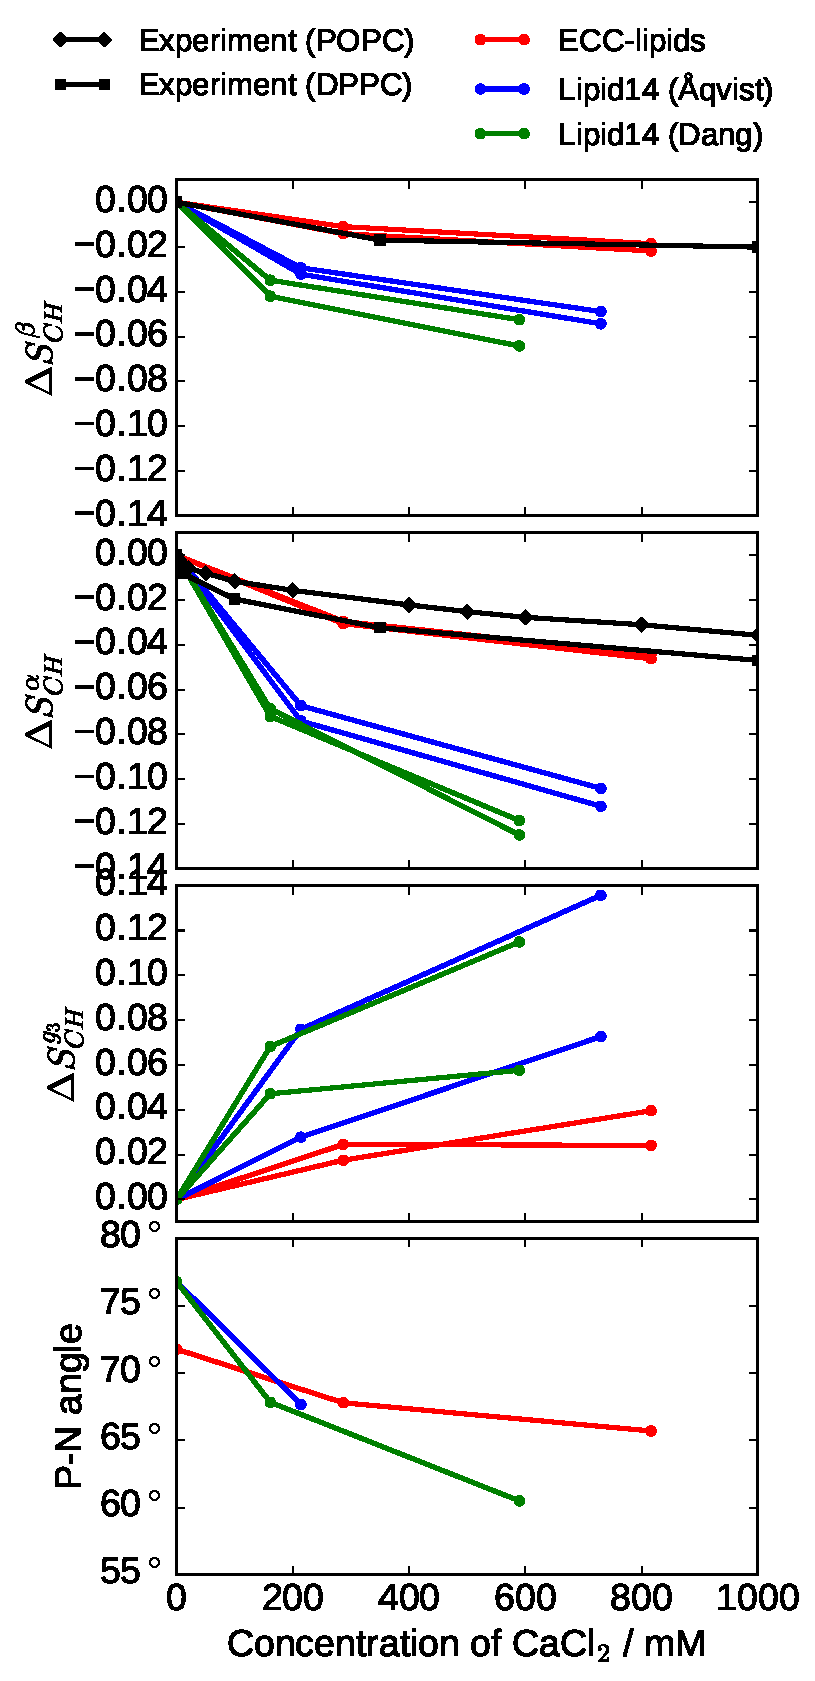
\includegraphics[width=8.0cm]{../Fig/ipython_nb/PN_angle_OrdPars-A-B-g3_L14-ECCL17_q80_sig89_CaCl.pdf}
  \caption{\label{fig:delta_ordPar_CaCl}
    Changes of the head group order parameters and P-N vector orientation of a POPC bilayer 
    as a function of the CaCl$_2$ concentration in bulk ($C_{ion}$)
    from simulations at 313 K together with experimental data 
    (DPPC (323\,K) \cite{akutsu81} and POPC (313\,K) \cite{altenbach84}). 
    The error estimate for bulk concentrations was approximately 10\,mM.
    Exception was the order of magnitude larger error in
    simulation with Lipid14 and ECC-ions due to the unconverged densities  (shown if Fig.~\ref{fig:cacl-dens}) because the 
    small simulation box. 
    Simulation data with Lipid14 and \AA{}qvist ion parameters at 298 K are taken directly from
    Refs.~\cite{lipid14POPC0mMNaClfiles,lipid14POPC350mMCaClfiles,lipid14POPC350mMCaClfilesNC}.
  }
  %Experimental values from \cite{akutsu81} for $g_3$ figure:
  %the value of $g_3$ order parameter of DPPC was -0.214 
  %in the absence of ions [average of two closely spaced splittings] and -0.211 in the presence
  %of 0.35 M CaCl$_2$ (at 59 Celcius). No effect of ions could be detected on DPPC bilayers labeled
  %at the C-2 segments of both fatty acyl chains.'' 
\end{figure}

Changes of the lipid bilayer head group order parameters extracted from simulations and
experiments \cite{akutsu81, altenbach84} are shown in Figs.~\ref{fig:delta_ordPar_NaCl}
and~\ref{fig:delta_ordPar_CaCl} as functions of NaCl or CaCl$_2$ concentrations.
As seen in Fig.~\ref{OrderParameterCHANGESsurf}, the order parameters decrease
proportionally to the amount of the bound positive charge.
These results can be thus used to compare the ion binding affinities to lipid bilayers between
simulations and experiments using the electrometer concept~\cite{seelig87, catte16}.

The experimentally measured small order parameter
changes with NaCl (Fig.~\ref{fig:delta_ordPar_NaCl}) 
are reproduced by the Lipid14 model simulated with \AA{}qvist ions.
However, the same combination of models overestimates the order parameter changes with CaCl$_2$ (Fig.~\ref{fig:delta_ordPar_CaCl}).
Replacing \AA{}qvist ions with ion parameters by Dang et al.~\cite{smith94, chang1999, dang2006}
or ECC-ions~\cite{martinek17, kohagen16, Pluharova2014} did not improve
the results~(Figs.~\ref{fig:delta_ordPar_NaCl} and \ref{fig:delta_ordPar_CaCl}).
In line with the previous work \cite{catte16}, the results suggest that improvements
in the lipid parameters are required to correctly describe the binding of cations to phospholipid bilayers.

The results from simulations combining the ECC-POPC with the ECC-ion models \cite{martinek17, kohagen16, Pluharova2014} exhibit a significantly improved behavior of the POPC head group order parameters as a function of NaCl or CaCl$_2$ concentrations, see Fig.~\ref{fig:delta_ordPar_NaCl} and Fig.~\ref{fig:delta_ordPar_CaCl}. Considering that we are also able to reproduce the experimental response in systems with known charge density (see above section \ref{section:boundCHARGE}), we conclude that our ECC model correctly reproduces the binding affinities of Na$^{+}$ and Ca$^{2+}$ ions to the POPC lipid bilayer. Furthermore, while the response of the glycerol backbone $g_3$ order parameter to CaCl$_2$ was significantly overestimated in the original Lipid14 model, the ECC-POPC model provides an improved agreement with experiment, as seen in Fig.~\ref{fig:delta_ordPar_CaCl}.
Also the changes of the P-N vector angle are too pronounced for the Lipid14 model,
for which the largest tilting toward water phase induced by a $780\,\mathrm{mM}$
CaCl$_2$ concentration is approximately 17$^{\circ}$. The corresponding value
for the ECC-POPC simulation is only 6$^{\circ}$ ($820\,\mathrm{mM}$ CaCl$_2$). 

Within the Lipid14 model, the overestimated changes in the lipid headgroup order parameter of POPC  as functions of the CaCl$_2$ concentration arise both from the overestimated binding affinity and the excessive sensitivity of the headgroup tilt to the bound positive charge. It is plausible to assume that the same applies to the other lipid models tested in a previous study~\cite{catte16}, which underlines the importance of validation of the lipid headgroup order parameter response to the bound charge. 

Finally, the ion binding affinities for the ECC-POPC model with different water models are compared in SI. In general, the performance of ECC-POPC with any of the tested water models is better than that of the original Lipid14 model, with the order parameter changes being slightly overestimated with the four-site water models and with TIP3P model.


\subsection{Binding affinities of Na$^+$ and Ca$^{2+}$ cations to the POPC membrane}
\label{sec:affinity}

\begin{table}[tb!]
  \caption{Bulk concentrations of Ca$^{2+}$ (C$_b$), relative surface excess of calcium with respect to water ($\Gamma_{Ca}^{\rm water}$),
    and the percetages of Ca$^{2+}$ bound to phosphate or carbonyl oxyges ($r^\mathrm{Ca^{2+}} _\mathrm{PO_4} $ and $r^\mathrm{Ca^{2+}} _\mathrm{O_{carb.}}$)
    in different POPC bilayer models. All systems have the same molar concentration of Ca$^{2+}$ with respect to water ($C_{ion}'$=350mM).
  \label{tab:binding}}
  \begin{tabular}{l|c c | c | c c}
    model                  & $C_{ion}'$ & $C_{ion}\,/\,\mathrm{mM}$ & $\Gamma_{Ca}^{\rm water} \,/\, \mathrm{nm}^{-2}$  & $r^\mathrm{Ca^{2+}} _\mathrm{PO_4} $ & $r^\mathrm{Ca^{2+}} _\mathrm{O_{carb.}} $ \\
    \hline
    ECC-POPC             &  350  &  $280\pm 10 $  &  $0.06 \pm 0.01 $                           &  99\%  &    25\%    \\
    Lipid14/\AA{}qvist     &  350  &  $210\pm 10 $  &  $0.13 \pm 0.01 $                          & 100\%  &    37\%     \\
    Lipid14/Dang           &  350  &  $160\pm 10 $  &  $0.23 \pm 0.03 $                            & 100\%  &    14\%    \\
    Lipid14/ECC-ions       &  350  &  $120\pm 100$  &  $0.35 \pm 0.11 $                         & 100\%  &    23\%    \\
%Average no. of bound cations:
%L14+Aqvist: all:22.7, phos:22.7, carb:8.5
%L14+Dang:   all:29.2, phos:29.2, carb:4.0
%L14+ECC-ion:all:37.7, phos:37.7, carb:8.5
  \end{tabular}
\end{table}

Binding affinities of Ca$^{2+}$ ions to a POPC bilayer in different simulation models were quantified by calculating the relative surface excess of calcium with respect to water molecules, $\Gamma_{\rm ion}^{\rm water}$, from Eq.~\ref{surfexcess}.
The values of $\Gamma_{\rm ion}^{\rm water}$
from different simulations with the same molar concetration of cations with respect
to water ($C_{ion}'$=350mM) are shown in Table~\ref{tab:binding}.
As expected from the changes of the lipid headgroup order parameters in Fig.~ \ref{fig:delta_ordPar_CaCl}, the relative surface excess of calcium, $\Gamma_{\rm Ca}^{\rm water}$ = 0.06~nm$^{-2}$, is significantly smaller for the ECC-POPC model than for the other models, 0.13--0.35~nm$^{-2}$.
Interestingly, the calculated relative surface excess of \ce{NaCl} at $1\,\mathrm{M}$ concentration (ECC-ions~\cite{Pluharova2014}) using our ECC-POPC model is not only quantitatively but also qualitatively different from \ce{CaCl2} having actually a negative value of $\Gamma_{Na}^{water} = -0.11 \pm 0.01) \rm{nm}^{-2}$ (Fig.~\ref{fig:cacl-dens}. This 
means that on average water molecules are preferred to sodium and chloride ions at the membrane-water interface.  
This is in contradiction with most of the available lipid force fields, which predict a small but positive surface excess of sodium at PC lipid bilayers \cite{catte16}.

\begin{figure}[htbp!]
  \centering
  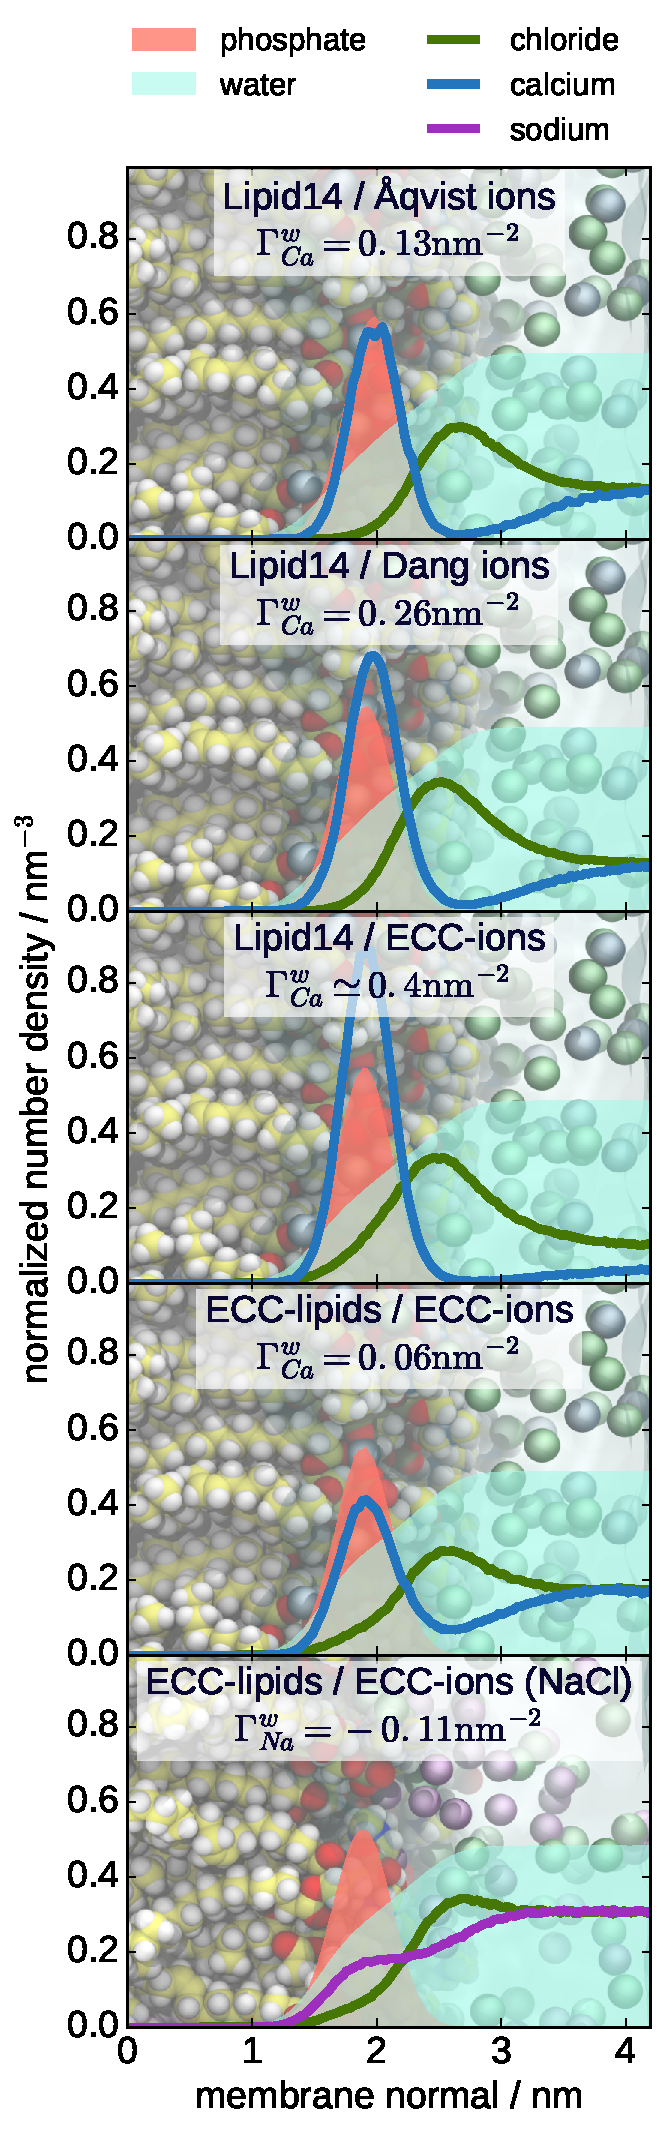
\includegraphics[height=19.5cm]{../Fig/ipython_nb/density_profiles_ca_cl_wat_phos_models-compar.pdf}
  \caption{\label{fig:cacl-dens}
    Number density profiles of \ce{Ca^{2+}}, \ce{Na^{+}} and \ce{Cl^-} along membrane normal axis
    for different force fields.
    In order to visualize the density profiles with a scale comparable to the profile of \ce{Ca^{2+}}, 
    the density profiles of~\ce{Cl^-} and \ce{Na^{+}} ions are divided by 2, and
    the density profiles of phosphate groups and water are divided by 5 and 200, respectively. 
    All simulations with \ce{CaCl2} shown here have the same molar concentration of ions in water ($C_{ion}'$=350~mM).
    The simulation with \ce{NaCl} has $C_{ion}'$=1000~mM.
    }
\end{figure}

\subsection{Molecular interactions between Na$^+$ or Ca$^{2+}$ cations and POPC oxygens}
We analyzed the ratio of the number of calcium cations bound to either phosphate or carbonyl moieties and the total number of bound cations in our POPC bilayers as done previously in Ref.~\citenum{javanainen17}. A maximum distance of 0.3~nm from any lipid oxygen is used to define a bound calcium. The results from ECC-POPC simulation in Table~\ref{tab:binding} show that almost all (99\%) of the bound Ca$^{2+}$ ions are in direct contact with phosphate oxygens. From these ions, only one third (32\%) also interacts with the carbonyl oxygens, while the interaction of calcium ions with carbonyl oxygens only is rare (1\%). The most abundand interaction scenarios between Ca$^{2+}$ ions and phosphate oxygens are visualized using the probability density isocontours in Fig.~\ref{fig:volmaps}. While higher concentrations of \ce{CaCl2} increase the number of contacts per lipid, the distribution of contacts between phosphate and carbonyl oxygens is not affected.

\begin{figure}[tb!]
  \centering
  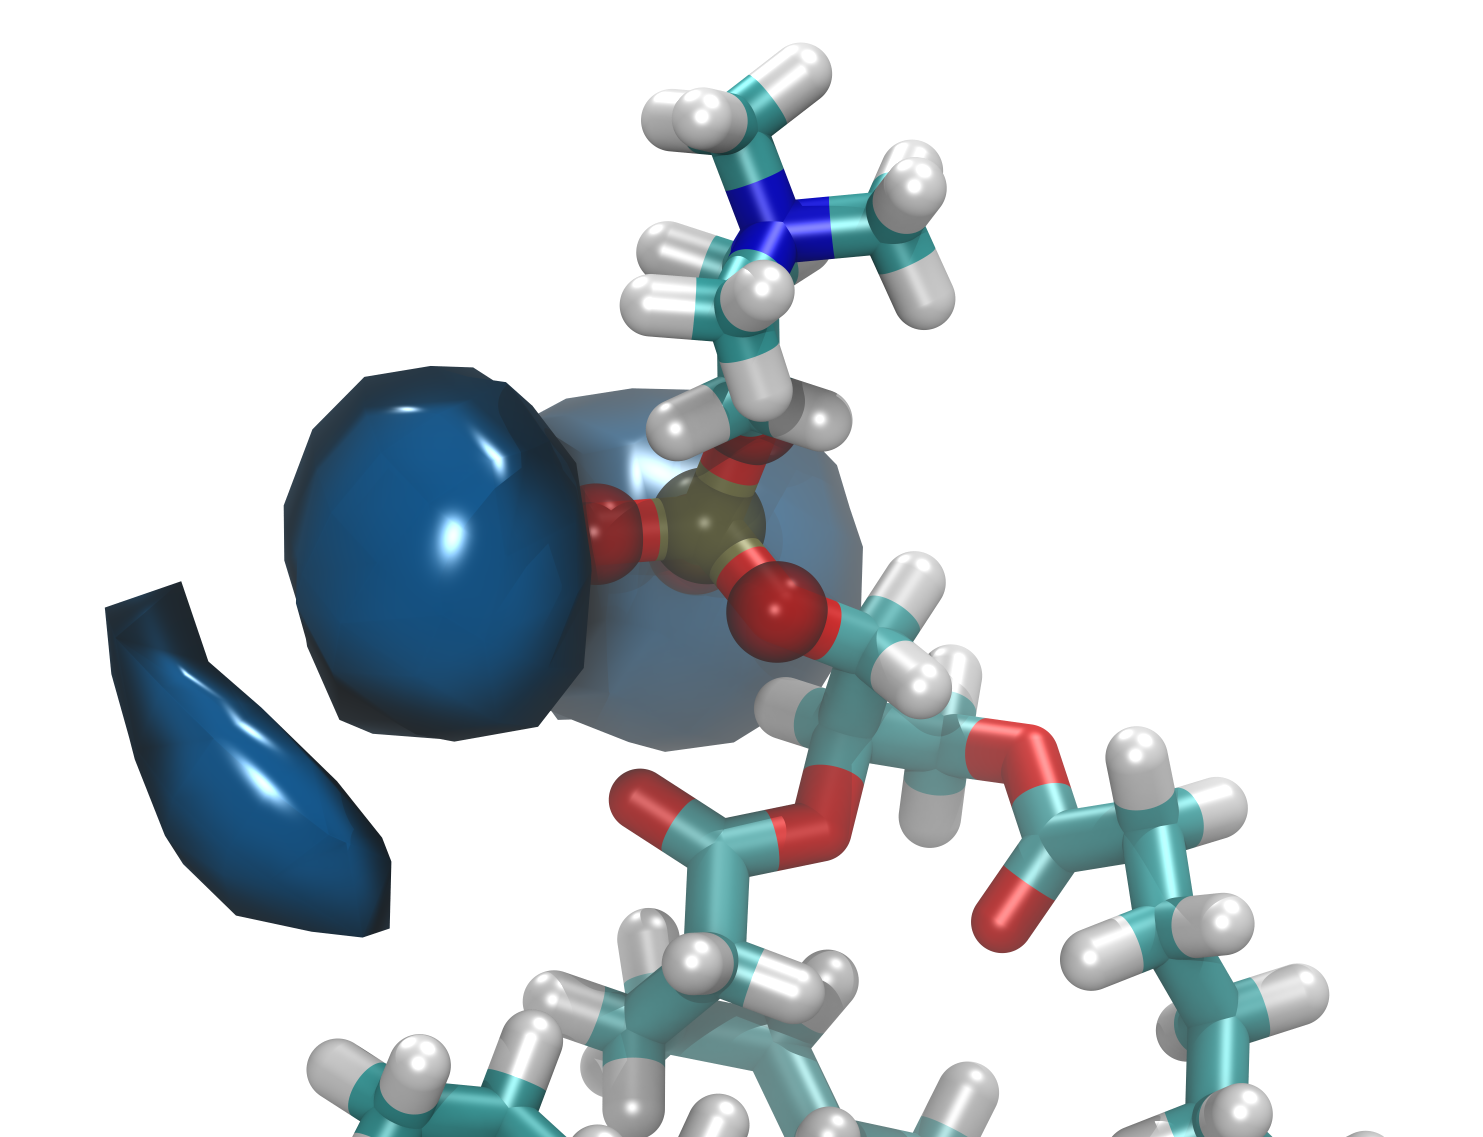
\includegraphics[width=8.0cm]{../Fig/volmap_resid10_Ca_Cl_PO4Cent.png} %\\
%  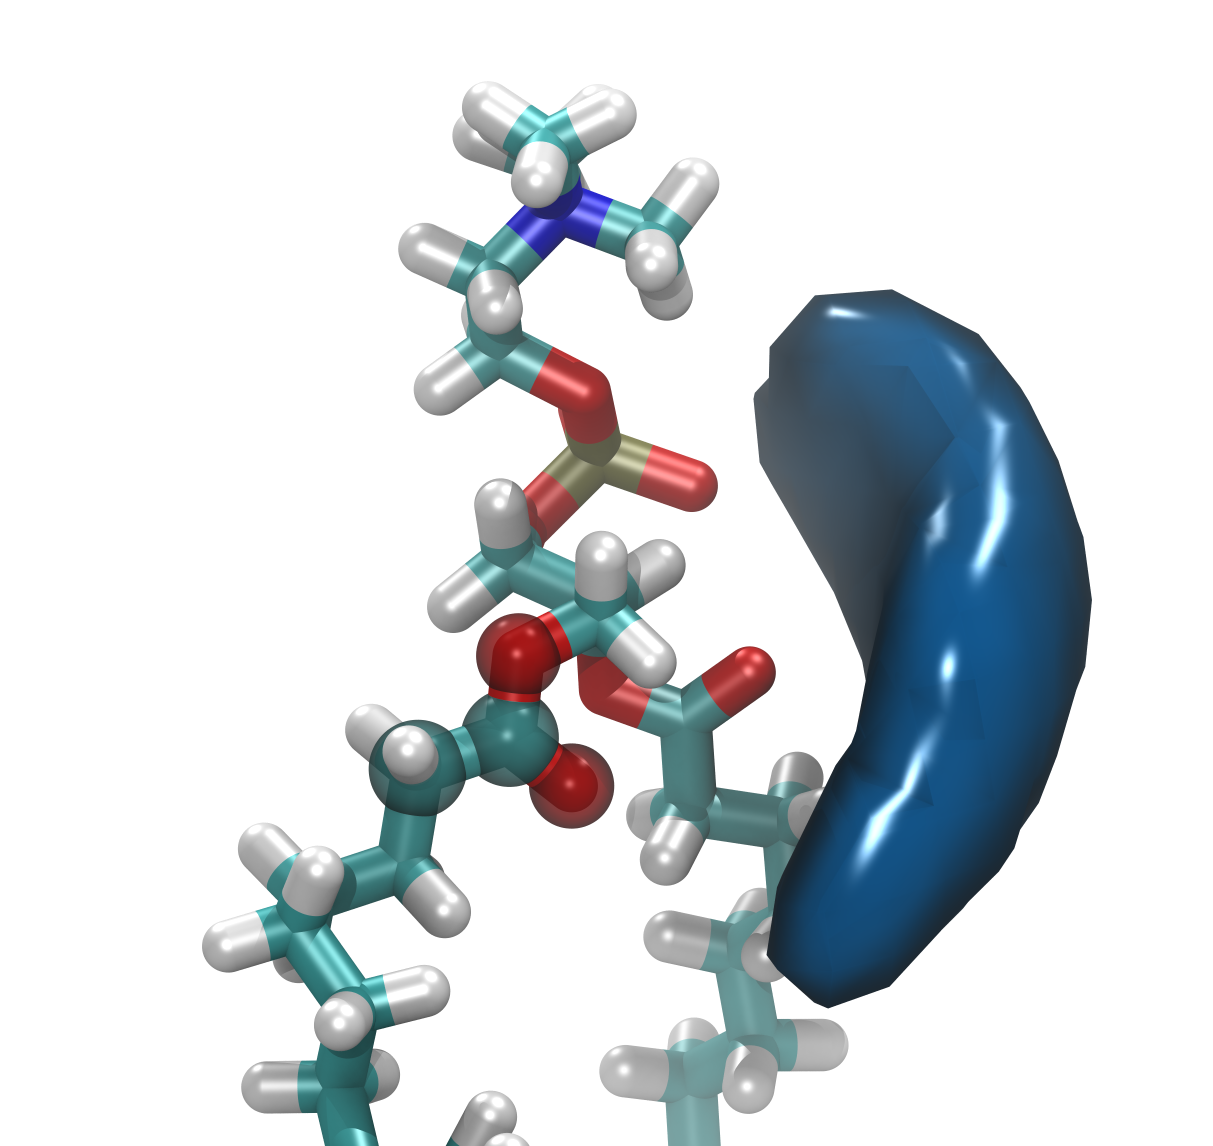
\includegraphics[width=4.0cm]{../Fig/volmap_resid10_Ca_Cl_sn1Cent.png}
%  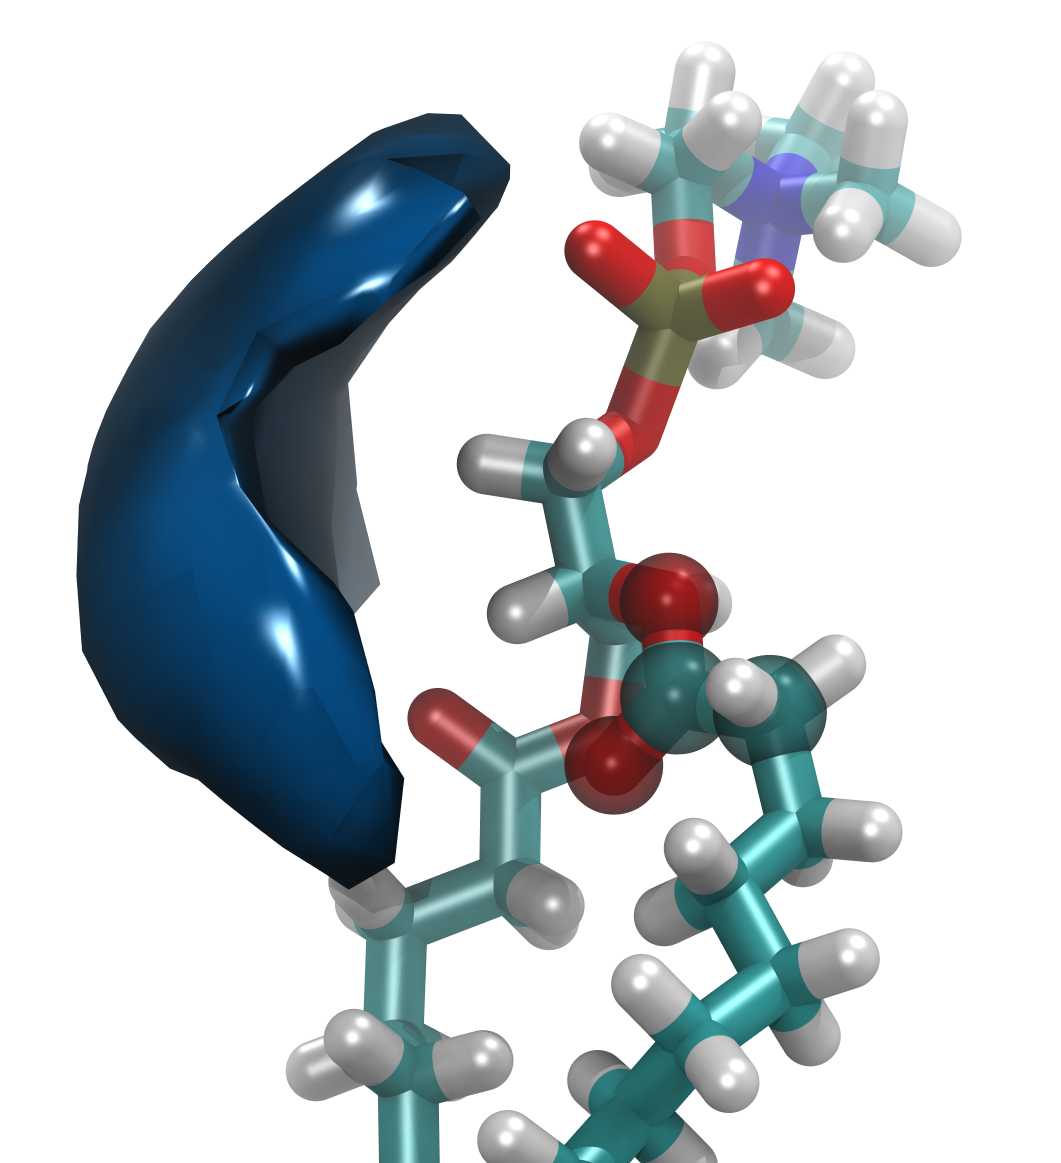
\includegraphics[width=3.6cm]{../Fig/volmap_resid10_Ca_Cl_sn2Cent.png}
  \caption{\label{fig:volmaps}
      Isocontours of probability density of \ce{Ca^{2+}} with respect to 
      the phosphate oxygens of POPC from ECC-POPC simulation.
      The probability density was evaluated around a single lipid, 
      after its strucutral alignment using only phosphate group. 
      %moiety, side chain 1 carbonyl group and side chain 2 carbonyl group.
      %Shown contours suggest that the dominant contribution 
      %to \ce{Ca^{2+}} binding comes from the phosphate oxygens,
      %whereas the interactions with any of the two carbonyl groups are considerably milder.
  }
  \todo{The figure should be updated as discussed last week.}
\end{figure}

Even though \ce{Na+} ions do not bind strongly to a POPC bilayer, they still interact mostly with its oxygen moieties. The results from a simulation at a $1\,$M \ce{NaCl} concentration show that 55\% of \ce{Na+} ions at the bilayer interact with phosphate oxygens of POPC only and 20\% with carbonyl oxygens only, with the remaining 25\%, is interacting with both negatively charged groups.

In conclusion, the results suggest that calcium ions bind specifically to the phosphate oxygens, occasionally interacting also with the carbonyls of the PC lipids. This is in a qualitative agreement with previous conclusions from several experimental and computational studies~\cite{hauser76, hauser78, herbette84, cevc90, binder02}. However, the present results suggest, in
agreement with experiments, an overally weaker binding to the bilayer, in particular with a lower relative binding affinity to the carbonyls than inferred from previous MD simulation studies~\cite{bockmann03, bockmann04, melcrova16, javanainen17}. Sodium ions, which do not exhibit any appreciable affinity for the bilayer, also interact primarily with phosphate oxygens of the POPC, but in contrast to calcium, the interactions purely with carbonyls are also significant.


\subsection{Binding stoichiometry of \ce{Na+} and \ce{Ca^{2+}} cations to POPC membrane}

%Binding probability:
%\ce{Ca2+} complex with \\
%1 POPC - 13\% -- 30\% \\
%2 POPC - 18\% -- 42\% \\
%3 POPC - 12\% -- 28\% \\

Simple binding models have been used previously to interpret the same experimental data \cite{altenbach84,macdonald87} as employed in this work to validate the simulation models (Fig.~\ref{fig:delta_ordPar_CaCl}). In particular, NMR data concerning the PC headgroup order parameters response and atomic absorption spectra were explained best using a ternary complex binding model with a binding stoichiometry of one \ce{Ca^{2+}} per two POPC lipids~\cite{altenbach84}. Nevertheless, a Langmuir adsorption model assuming a \ce{Ca^{2+}}:POPC stoichiometry of 1:1 also provided a good fit to the experimental data when considering \ce{CaCl2} at low concentrations only~\cite{macdonald87}.


In this work, we reproduce the same experimental data used to infer binding stoichiometries employing our ECC-POPC model. Thanks to our simulations, we have a direct access to atomistic details of the binding stoichiometry without a need for any binding model as employed for interpreting in experiments~\cite{altenbach84, macdonald87}. To evaluate the relative propensities for each of the stoichiometric complexes (i.e.,~1~Ca$^{2+}$:~n~POPC), we calculated for each bound Ca$^{2+}$ the number of POPC molecules within a distance of 0.3~nm.
Results from the POPC bilayer simulation with a 285~mM bulk concentration of CaCl$_2$ are shown in Fig.~\ref{fig:cacl_complexes}.
We found the largest propensity for the 1:2 complex (41\%), with probabilities of complexes with the stoichiometries of 1:1~(25\%)~and 1:3~(34\%)~being only slightly lower. This suggests a more complex binding model than considered in a simple 1:2 ternary complex model previously. Nevertheless, with a broad brushstroke, the simulation data can be viewed such that one calcium binds to two lipids on average, because the probabilities of the complexes with 1 or 3 lipids are almost equal to each other  (and complexes with more than three lipids per one calcium ion were not observed). This probably explains why the simple the ternary complex model fits adequately the experimental data, as well as the ECC-POPC simulation results (see Fig.~S3 in SI).

\begin{figure}[tb!]
  \centering
  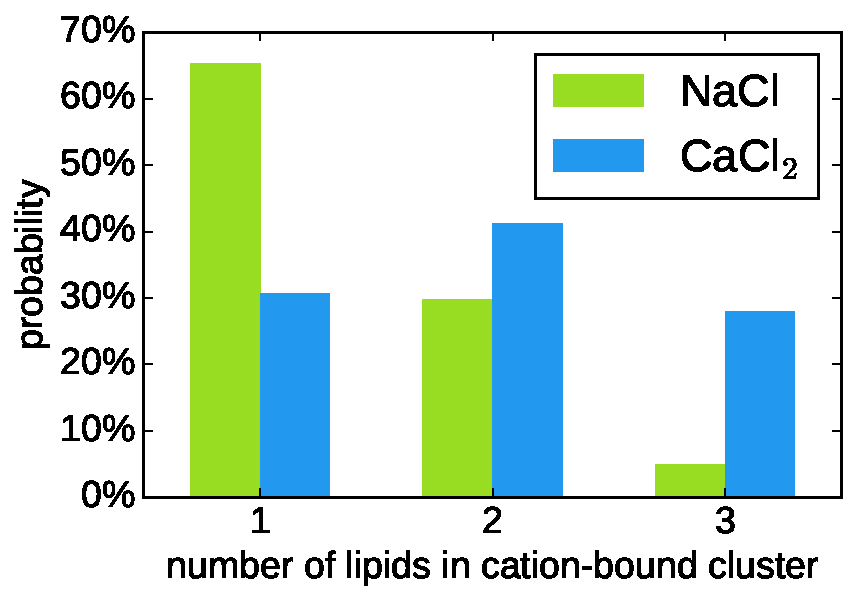
\includegraphics[width=8.0cm]{../Fig/ipython_nb/stoichiometry_NaCl-CaCl2_comparison_Ecc-lipids.pdf} \\
  \caption{\label{fig:cacl_complexes}
      Relative probabilities of existence of \ce{Na^{+}} or \ce{Ca^{2+}} complexes
      with a certain number of POPC lipids. 
      \ce{Na^{+}} complexes were evaluated from the simulation with 1~M concentration;
      and \ce{Ca^{2+}} complexes were evaluated from the simulation with 287~mM concentration.
  }
\end{figure}

The probabilities of different complexes formed by \ce{Na+} ions and POPC
analyzed from the simulation with the ECC-POPC model at $1\,$M concentration of NaCl are also 
shown in Fig.~\ref{fig:cacl_complexes}. In contrast to calcium, the
probability is largest (67\%) for 1:1 complex, significantly smaller (29\%)
for 1:2 complexes and very small (4\%) for 1:3 of \ce{Na+}:POPC complexes.




\subsection{Residence times of \ce{Na+} and \ce{Ca^{2+}} cations in the POPC membrane}

Equilibration of \ce{Ca^{2+}} ions at a POPC bilayer in MD simulations is a microsecond time scale process with current force fields, such  as CHARMM36 and Slipids force fields~\cite{javanainen17}. This suggests that at least several microseconds are required to reach the ion binding/unbinding equilibrium.
To quantify the exchange of ions between the membrane and aqueous solution in simulations, we evaluated residence times of ions bound to the membrane. Within our analysis, an ion is considered to be bound when it is within 0.3~nm from any oxygen atom belonging to a POPC molecule.

The histograms of residence times of \ce{Ca^{2+}} in a POPC bilayer ($C_{ion}'$ = 450~mM) from simulations with 
ECC-POPC and CHARMM36 (simulation from Refs.~\citenum{javanainen17,zenodo.259376}) are shown in Fig.~S4 in SI.
In the CHARMM36 simulation, a significant number of the calcium ions is bound to the membrane for the whole length of the trajectory (800~ns).
In contrast, at least an order of magnitude faster bound/unbound calcium exchange is observed within the ECC-POPC model,
where 90\% of the \ce{Ca^{2+}} residence times to a POPC membrane are shorter than $60\,\mathrm{ns}$. The longest observed
residence time is around 150~ns, which is below the total length of the simulation used for analysis, i.e., 200~ns.
Note that these results are in line with the experimental estimate that the residence time of \ce{Ca^{2+}} at each PC
headgroup is of the order of $10\,\mu\mathrm{s}$~\cite{altenbach84}. Note that the exchange of \ce{Na+} ions at the POPC membrane
is yet another order of magnitude faster, with 90\% of the residence times smaller than~1~ns and the longest residence time being~6~ns.

In summary, the results from the ECC-POPC model suggest that the exchange of calcium between the POPC bilayer and the solvent occurs within the $\sim$100~ns timeframe, which is significantly faster than observed in simulations emloying most of the presently available lipid models~\cite{javanainen17}. Sodium cations exhibit an even more rapid exchange between the membrane and the aqueous solution. Our results suggest that simulations with a length of several hundreds of nanoseconds are sufficient to simulate alkali and alkali earth ion binding to phospholipid bilayers in equilibrium when realistic force fields are used. This has not been the case with previous lipid force fields, which overestimate the binding strength of the sodium and, in particular,  calcium cations \cite{javanainen17, catte16}.


\section{Conclusions}

In this study, we employed the electrometer concept to demonstrate that the binding of \ce{Na^+} and \ce{Ca^2+} ions to a POPC lipid bilayer can be accurately described within a force field MD simulation, provided that electronic polarization is implicitly included via the electronic continuum correction~\cite{leontyev11}. This ECC-POPC model is built upon the Lipid14 POPC model~\cite{dickson14} by scaling the partial charges by a factor of 0.8 and reducing the Lennard-Jones radii by a factor of 0.89 for the headgroup, glycerol backbone, and carbonyl atoms. While the structural details of a POPC lipid bilayer in pure water simulated with the newly developed ECC-POPC model agree with experiments with an accuracy comparable to the other state of the art lipid models, the new model in addition reproduces the experimental lipid head group order parameter responses to a cationic surfactant, NaCl, and CaCl$_2$ at varying concentrations. It thus represents a significant improvement over currently available lipid models, which tend to overestimate cation binding affinities~\cite{catte16}. 

The good agreement with experiments enables us to interpret NMR experiments with atomistic details using MD simulations with the ECC-POPC model. In line with previous interpretations of the experimental data \cite{hauser76,hauser78,herbette84,binder02}, Ca$^{2+}$ ions interact mainly with phosphate oxygens, with interactions to the carbonyls being of a secondary importance. However, the stoichiometry of calcium binding is significantly more complicated than the simple ternary complex model, used to interpret NMR data previously, within which one calcium binds to two POPC molecules~\cite{altenbach84}. While complexes with one calcium ion bound to two lipids are the most probable also in the ECC-POPC model, complexes of one or three lipids per one calcium were observed to be relatively abundant and also almost equally likely to occur. While the success of the simple ternary complex model in fitting NMR data is understandable based on the simulation results, it cannot capture the detailed nature of calcium binding to phospholipid bilayers observed in the present simulation.

Accurate description of cation binding to POPC bilayer paves the way for simulations of complex biochemical systems at cellular membranes with realistically described electrostatic interactions, including a mean-field account for electronic polarization effects. To this end, the compatibility of the ECC-POPC model with existing models for proteins and other biological molecules needs to be verified and, if necessary, further adjustments following the ECC concept to the force fields of the biomolecules interacting with the lipids should be made.


This work can be reached as a repository containing all data at \url{zenodo.org:\dots\dots\dots}.


% If you have acknowledgments, this puts in the proper section head.
\begin{acknowledgments}
% Put your acknowledgments here.
P.J. acknowledges support from the Czech Science Foundation (grant no. 16-01074S) 
and from the Academy of Finland via the FiDiPro award.
J.K. acknowledges support from the Czech Science Foundation, Project No. 15-12386S.
Computational resources were supplied by the Ministry of Education, Youth and Sports
of the Czech Republic under the Projects CESNET (Project No. LM2015042) and CERIT-Scientific
Cloud (Project No. LM2015085) provided within the program Projects of Large Research,
Development and Innovations Infrastructures.
O.H.S.O. acknowledges financial support from
Integrated Structural Biology Research Infrastructure of
Helsinki Institute of Life Science (Instruct-HiLIFE).
\end{acknowledgments}

%\newpage
%\appendix

% Create the reference section using BibTe
\bibliography{refs.bib}

\listoftodos

\end{document}
%
% ****** End of file aiptemplate.tex ******
